\documentclass[12pt]{article}

% 导入中文支持的包
\usepackage[UTF8]{ctex} % ctex 包支持中文处理

% 设置页面布局(可选)
\usepackage[a4paper,margin=1in]{geometry}

% 导入常用包(根据需要添加)
\usepackage{amsmath, amssymb} % 数学公式
\usepackage{graphicx} % 插入图片
\usepackage{hyperref} % 超链接
\hypersetup{
    colorlinks=true, % 激活链接颜色
    linkcolor=blue, % 文档内部链接颜色,适用于图、表在文中的引用
    citecolor=blue, % 文献引用链接颜色,适用于文中参考文献引用
    urlcolor=blue  % 外部URL链接颜色,适用于参考文献添加超链接
}
\usepackage{xcolor} % 颜色支持

% 标题和作者信息(可选)
\title{颅内压生理学和脑脊液动力学的仿体模型}
\author{王成}
\date{\today}

\begin{document}

% 标题
\maketitle
\newpage

% 目录(可选)
% \tableofcontents
% \newpage

% 正文
\begin{center}
    \section*{摘要}
\end{center}

我们在此描述了一种新颖的与颅腔等大的仿体模型,并给出了其验证过程。包括脑室、池区和蛛网膜下腔在内的脑脊液区域由核磁共振成像获得。
脑的机械特性和颅脊顺应性是基于已发表的数据设定的。实现了对脑脊液流动进行整体和脉动的生理建模。通过将模型中的流量和压力测量结果与健康受试者的体内数据进行比较来验证模型有效性。
脑室内记录的生理颅内压平均为10 mmHg,脉冲峰值幅度为0.4 mmHg。在大脑导水管和蛛网膜下腔中分别测得脑脊液流速峰值为0.2和2 ml/s。
本模型是一种首次尝试在体外模拟生理颅内动力学的方法。在此,我们描述了模型的设计和制造,操作参数的定义和实现,以及所模拟动力学的验证。

索引术语——解剖模型,顺应性,蛛网膜下腔(SAS),脑室系统。

\section*{\uppercase\expandafter{\romannumeral1}.引言}

脑脊液(CSF)有助于中枢神经系统(CNS)的体内平衡。在颅腔中,由于受到大气压强的作用,脑脊液被局限在脑室和蛛网膜下腔(SASs)中。
脑脊液通过浮力支撑大脑,保护其免受冲击,输送营养物质和神经内分泌物质,并清除代谢废物。

CSF动力学的变化与多种疾病有关。例如,脑积水和脊髓空洞症已被证明与CSF总体流动及脉动的紊乱有关。然而,这些关系的具体细节尚不清楚。

颅内动力学模型可以提高对中枢神经系统病理生理学的理解。集总参数和计算流体动力学(CFD)模型均已用于表征CSF空间以及主要颅内动脉的动力学特征。
集总参数方法特别适合用于颅内动力学的整体经验描述。相应的模型参数,如脑脊液流出阻力和压力-体积指数,在过去的十年中已成为临床实践中的标准。
另一方面,CFD模型可以用于获取通过测量无法获得的空间分辨流动信息。

然而,无论是集总参数模型还是CFD模型都未被证明是开发及优化颅腔动力学相关医疗器械的理想选择。
例如,用于治疗脑积水的脑脊液分流器根据ISO 7197标准通过实验方式进行测试以评估液压阻力。
然而,除了伦理问题,比起小鼠、老鼠或兔子,尤其是当使用诸如狗、山羊或猴子等脑内动力学与人类更为接近的大型动物时,实验成本将会非常昂贵。
体外模型代表了第四种可能有助于研究中枢神经系统病理生理学的模型类型。解剖细致和简化的模型都已被用于验证MRI序列、脑力学的计算模型,以及第三脑室中脑脊液流动。在脑损伤研究中,模型被用于研究组织对冲击的反应。
据我们所知,仅有一个关于脊柱脑脊液空间中流体和压力动态的模型被报道过;该模型被用于理解脊髓空洞症。

颅内空间的仿体模型有可能减少、改进,并在较小程度上取代动物模型用于分流器和其他神经外科器械的测试。
实现此类应用的一个重要步骤是复制健康状态下的颅内动力学。我们在此展示了首创的颅内腔体仿体模型,该模型能够再现生理性的脑脊液和压力动态。
我们报告了幻影的设计、开发及与文献中描述的体内数据的验证,显示这种建模方法可以促进对颅内动力学的理解。

\section*{\uppercase\expandafter{\romannumeral2}.材料与方法}

\subsection*{A. 脑脊液和脑室系统}
我们使用以下方法在硅胶大脑中构造了一个脑室系统:对 27 岁健康男性志愿者采集的 MRI 数据进行3D重建,为设计模型的脑室区域提供了解剖学参考。
将脑室系统简化以获得适合铸造的矢状对称性:利用计算机辅助设计(CAD)软件(NX 7.5,西门子PLM软件,美国德克萨斯州普莱诺)将侧脑室合并为单一脑室表示;Monro孔被统一为通向第三脑室的单一连接器;Luschka孔和Magendie孔也被合并为单一通道。
这个简化的脑室区域的负模通过3D打印在Eden350V光聚合物打印机(Objet Geometries公司,美国马萨诸塞州比勒里卡市)上制造为两个矢状对称的半部分。

在获得脑室空间的正像(见第II-B节)后,将一个内径为2毫米的硅胶管插入到大脑导水管中,以避免其在模拟体构建期间发生形变。
为了模拟脑室中的脑脊液生成,在脑室系统的顶部建立了一个接入端口。这个接入端口也用于脑脊液空间的初步填充。在大脑导水管的顶部和底部建立了两个压力感应接入点。
改进的脑室系统如图\ref{fig:ventricular_system}所示,简化的效果在第IV节讨论。
\begin{figure}[h]
    \centering
    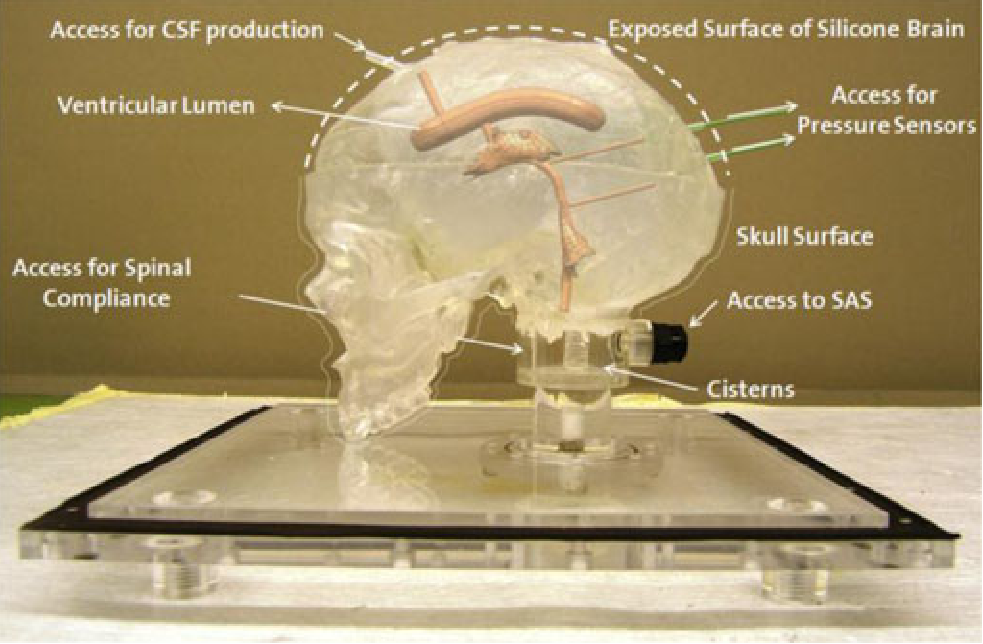
\includegraphics[width=0.7\textwidth]{Figures/1.png}
    \caption{模型的颅域。硅质大脑被容纳在塑料人类颅骨内。简化脑室系统的腔内显示为CAD模型的叠加。}
    \label{fig:ventricular_system}
\end{figure}
\subsection*{B.大脑和颅骨}
使用Sylgard 527,A&B绝缘硅胶(陶氏康宁,密歇根州米德兰)制成了一颗真人大小的硅胶大脑。先前的研究表明,这种材料在静态变形和动态加载高达10Hz时具有类似大脑的机械行为。
硅胶是围绕两个脑室负半部分铸造的。
固化后,负片被移除,左右脑部件用相同的硅胶粘在一起。在脑室壁上涂上一层标准铸造硅胶,以防止在坍塌时粘连。

完整的大脑被放置在一个已经移除上部的塑料人类头骨模型内(3B Scientific,德国汉堡)(见图\ref{fig:ventricular_system})。
\begin{figure}[h]
    \centering
    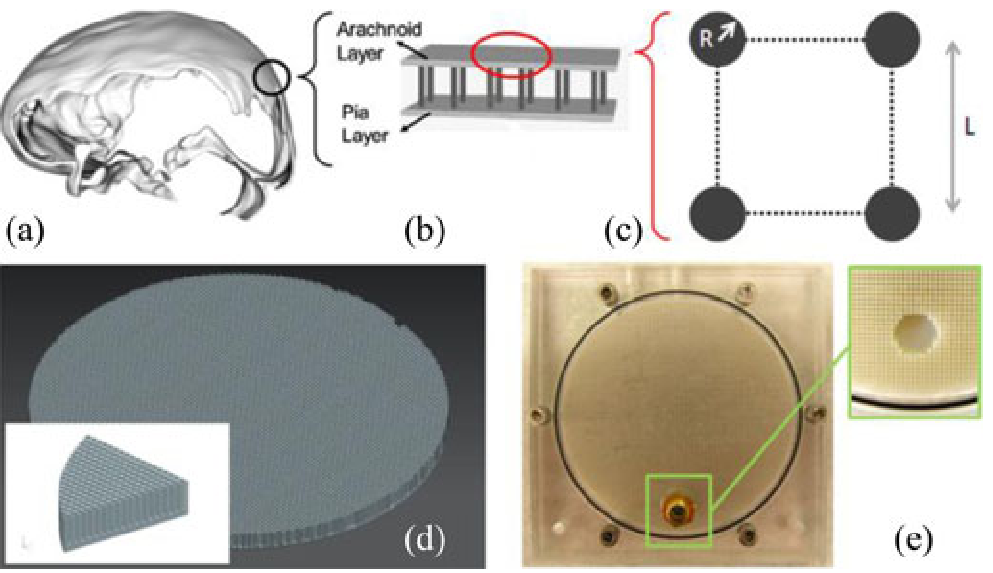
\includegraphics[width=0.6\textwidth]{Figures/2.png}
    \caption{SAS隔室设计。采用统一的模块化柱状结构以实现体内液力阻力值。 (a) SAS 宏解剖学。 (b) 理想化的柱状结构代表 SAS 微解剖学。 (c) 代表性单元格的顶视图。 (d) SAS 隔室的 CAD 设计。 (e) 3-D 打印的 SAS 表示和连接到模型的脑脊液池 (参见图 4)。}
    \label{fig:silicone_brain}
\end{figure}

\begin{figure}[h]
    \centering
    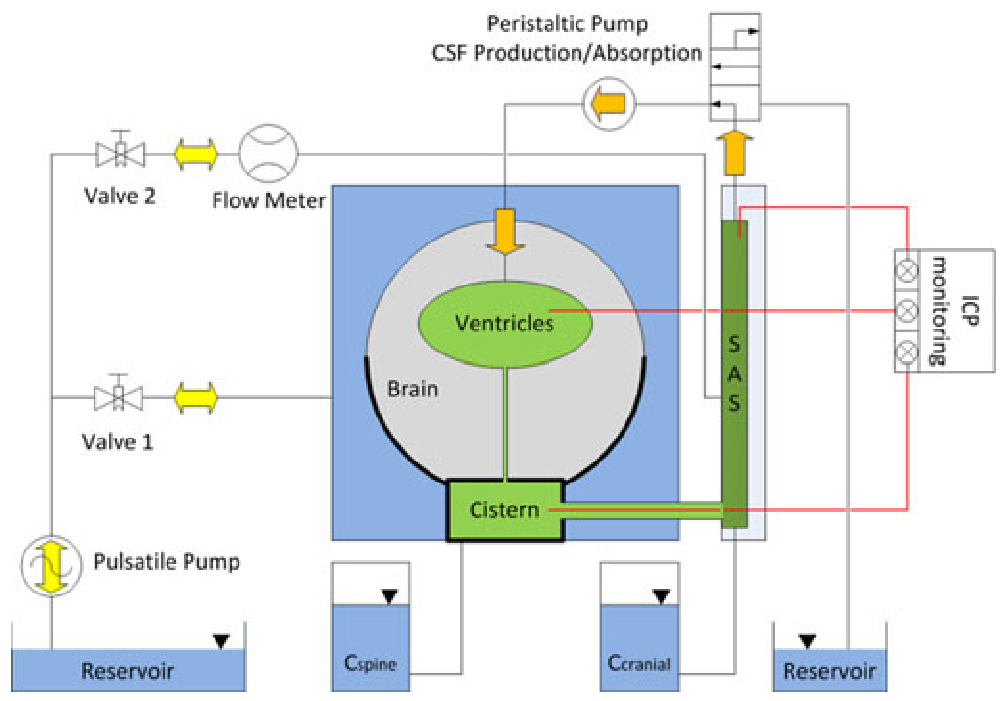
\includegraphics[width=0.7\textwidth]{Figures/3.png}
    \caption{仿真体设置示意图。脑室被包裹在硅胶大脑中,并连接到脑池和蛛网膜下腔。脑脊液产生和吸收速率可被控制。脑脊柱和颅脑顺应性单位分别连接到脑池和蛛网膜下腔。脉动流和颅内压在指示的位置监测。黑色三角形表示水-空气界面。}
    \label{fig:model_assembly}
\end{figure}
\subsubsection*{C.蓄水池与SAS}
脑脊液的整体流动起始于脑室,继续流向颅底的池,最终到达脊髓和皮质蛛网膜下腔(SAS),在那里大部分被重吸收至静脉血中。
SAS 的微观结构影响脑脊液动力学。微观结构的影响可以通过其水力阻力的空间平均和表示,而水力阻力与渗透率有关。
据报道,SAS 的渗透率范围在$10^{-9}$到$10^{-7}$平方米之间。我们使用了平行板之间的均质柱结构(见图\ref{fig:silicone_brain})来解释 SAS 的水力阻力。
在这样的结构中,渗透率$k$是柱半径$r$和空隙率$\varepsilon$的函数:
\begin{equation}
    \frac{k}{r^2} = \frac{\pi \varepsilon \left(1 - \sqrt{1 - \varepsilon}\right)^2}{24 \left(1 - \varepsilon\right)^{3/2}} \quad \text{and}
\end{equation}

\begin{equation}
    \varepsilon = \frac{V_{\text{fluid}}}{V_{\text{tot}}} = \frac{L^2 - \pi r^2}{L^2}
\end{equation}



\section*{\uppercase\expandafter{\romannumeral3}.结果}

\section*{\uppercase\expandafter{\romannumeral4}.讨论}




\end{document}
